\documentclass[conference]{IEEEtran}
\usepackage{amsmath,amssymb,amsfonts}
\usepackage{xcolor}
\usepackage{amssymb}
\usepackage{color}
\usepackage{pgfplots}
\usepackage{tikz}
\usetikzlibrary{positioning, decorations.pathreplacing, arrows.meta}

\begin{document}

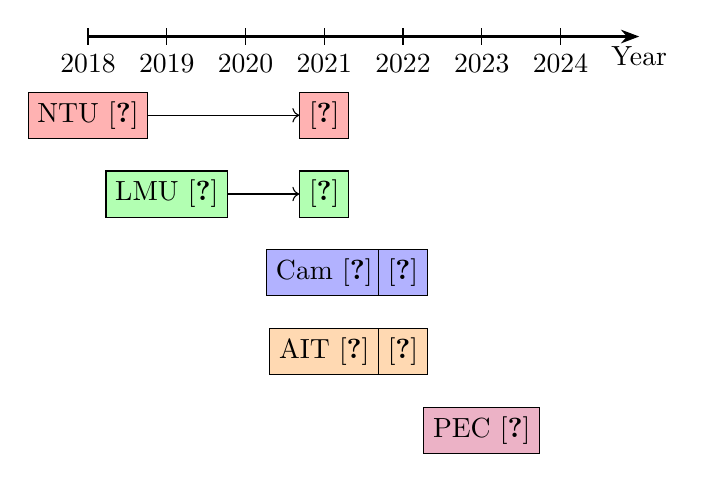
\begin{tikzpicture}
    % Draw the timeline
    \draw[thick, -Stealth] (0,0) -- (7,0) node[anchor=north] {Year};

    % Add years to the timeline (2018-2023)
    % Assuming each unit represents one year
    \foreach \x/\year in {0/2018, 1/2019, 2/2020, 3/2021, 4/2022, 5/2023, 6/2024} {
        \draw (\x cm,3pt) -- (\x cm,-3pt) node[anchor=north] {\year};
    }

    % Mark activities for Nanyang Technological University
    \node[draw, rectangle, fill=red!30] (NTU1) at (0,-1) {NTU \cite{tandoc_jr_defining_2018}};
    \node[draw, rectangle, fill=red!30] (NTU2) at (3,-1) {\cite{maronikolakis_identifying_2021}};

    % Mark activities for Ludwig-Maximilians-University of Munich
    \node[draw, rectangle, fill=green!30] (LMU1) at (1,-2) {LMU \cite{egelhofer_fake_2019}};
    \node[draw, rectangle, fill=green!30] (LMU2) at (3,-2) {\cite{maronikolakis_identifying_2021}};

    % Mark activities for Cambridge University
    \node[draw, rectangle, fill=blue!30] (Cam1) at (3,-3) {Cam \cite{osmundsen_partisan_2021}};
    \node[draw, rectangle, fill=blue!30] (Cam2) at (4,-3) {\cite{arora_generative_2022}};

    % Mark activities for Austrian Institute of Technology
    \node[draw, rectangle, fill=orange!30] (AIT1) at (3,-4) {AIT \cite{del_bimbo_automatic_2021}};
    \node[draw, rectangle, fill=orange!30] (AIT2) at (4,-4) {\cite{schutz_ait_fhstp_2022}};

    % Mark activities for Pôle d'excellence cyber (PEC)
    \node[draw, rectangle, fill=purple!30] (PEC1) at (5,-5) {PEC \cite{noauthor_podexcellence_2023}};

    % Connectors to indicate progression
    \draw[->] (NTU1) -- (NTU2);
    \draw[->] (LMU1) -- (LMU2);
\end{tikzpicture}

\end{document}